%(BEGIN_QUESTION)
% Copyright 2010, Tony R. Kuphaldt, released under the Creative Commons Attribution License (v 1.0)
% This means you may do almost anything with this work of mine, so long as you give me proper credit

Regn ut trykkene $P_1$ og $P_2$, anta at massetettheten til fluidet er 886.45 kg/m$^3$.

$$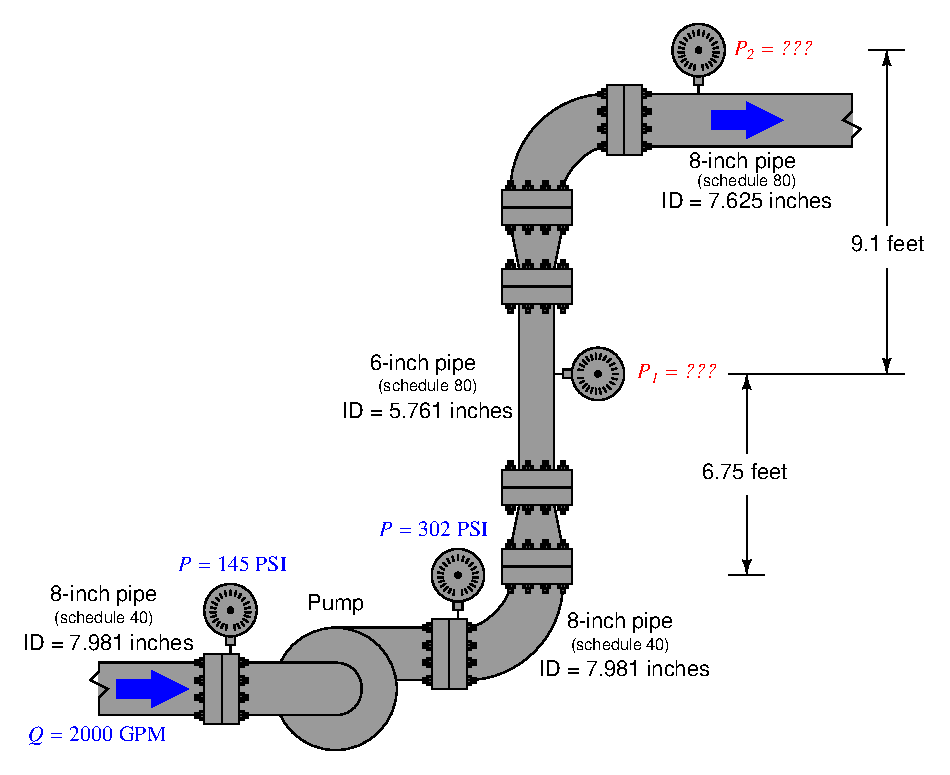
\includegraphics[width=15.5cm]{i00457x01.eps}$$

Kommenter også om Bernoullis ligning kan brukes til å sammenligne suge- og utløpstrykket til pumpen, gitt at disse to trykkene (145 og 302 PSI) er målt på rør med samme diameter, samme strømningsrate og svært lik høyde.

\underbar{file i00457}
%(END_QUESTION)





%(BEGIN_ANSWER)

$P_1$ = 296.77 PSI \hskip 30pt $P_2$ = 293.27 PSI

\vskip 10pt

Bernoullis ligning forutsetter at det ikke tilføres eller tapes energi mellom de to punktene som sammenlignes, og derfor {\it kan den ikke} brukes til å sammenligne pumpens suge- og utløpstrykk. Pumpen tilfører energi til fluidet som passerer gjennom den, og dermed er antakelsen om lik total energi i innløps- og utløpsstrøm ikke oppfylt.

%(END_ANSWER)





%(BEGIN_NOTES)


%INDEX% Physics, dynamic fluids: Bernoulli's equation

%(END_NOTES)
